\documentclass[11pt]{article}
\usepackage[margin=1in]{geometry}
\usepackage{graphicx}
\usepackage{booktabs}
\usepackage{enumitem}
\usepackage{hyperref}
\usepackage{parskip}
\usepackage{titlesec}
\usepackage{xcolor}
\usepackage{array}
\usepackage{tabularx}

\definecolor{questgreen}{RGB}{52, 199, 89}
\definecolor{darkgray}{RGB}{44, 44, 46}

\hypersetup{
    colorlinks=true,
    linkcolor=darkgray,
    urlcolor=darkgray,
}

\title{\textbf{Sidequest} \\ \large Interactive Applications --- Milestone 2 \\ \normalsize DS 5023}
\author{Thomas Blalock \and Jackson Kennedy \and Hudson Noyes \and Nathan Wan}
\date{April 3, 2026}

\begin{document}
\maketitle

\tableofcontents
\newpage

% =============================================================================
\section{Page Architecture Plan}
% =============================================================================

\subsection{Page List}

Sidequest is a proximity-based social activity app built for college-aged adults like Leo Vance, our M1 persona, who wants to spontaneously discover or host low-stakes local activities without the friction of formal event platforms. The app is organized into five pages:

\begin{table}[h!]
\centering
\begin{tabularx}{\textwidth}{>{\bfseries}l X l}
\toprule
Page & Purpose & User Goal (M1) \\
\midrule
Discovery Feed & Browse nearby quests, filter by time/distance/category, and join in one tap & Find an activity right now with minimal effort \\
\addlinespace
Host a Quest & Fill out a short form to publish a new activity to the local feed & Broadcast a spontaneous activity without bureaucracy \\
\addlinespace
My Quests & View, manage, and cancel all active and past quests & Know what you have committed to and easily back out \\
\addlinespace
Group Chat & Message quest members without exchanging phone numbers & Coordinate with strangers safely before meeting in person \\
\addlinespace
Quest Detail & See the full description, attendee list, and a large join/leave button for any quest & Get all the context needed to commit or pass on an activity \\
\bottomrule
\end{tabularx}
\caption{Page list with purpose and connection to Leo's goals.}
\end{table}

\subsection{Sketches and Design Annotations}

Each page was sketched before implementation. Sketches are included below. The goal of the sketching phase was to establish layout and navigation quickly before committing to any Streamlit-specific component choices.

\subsubsection{Discovery Feed}

\begin{center}
    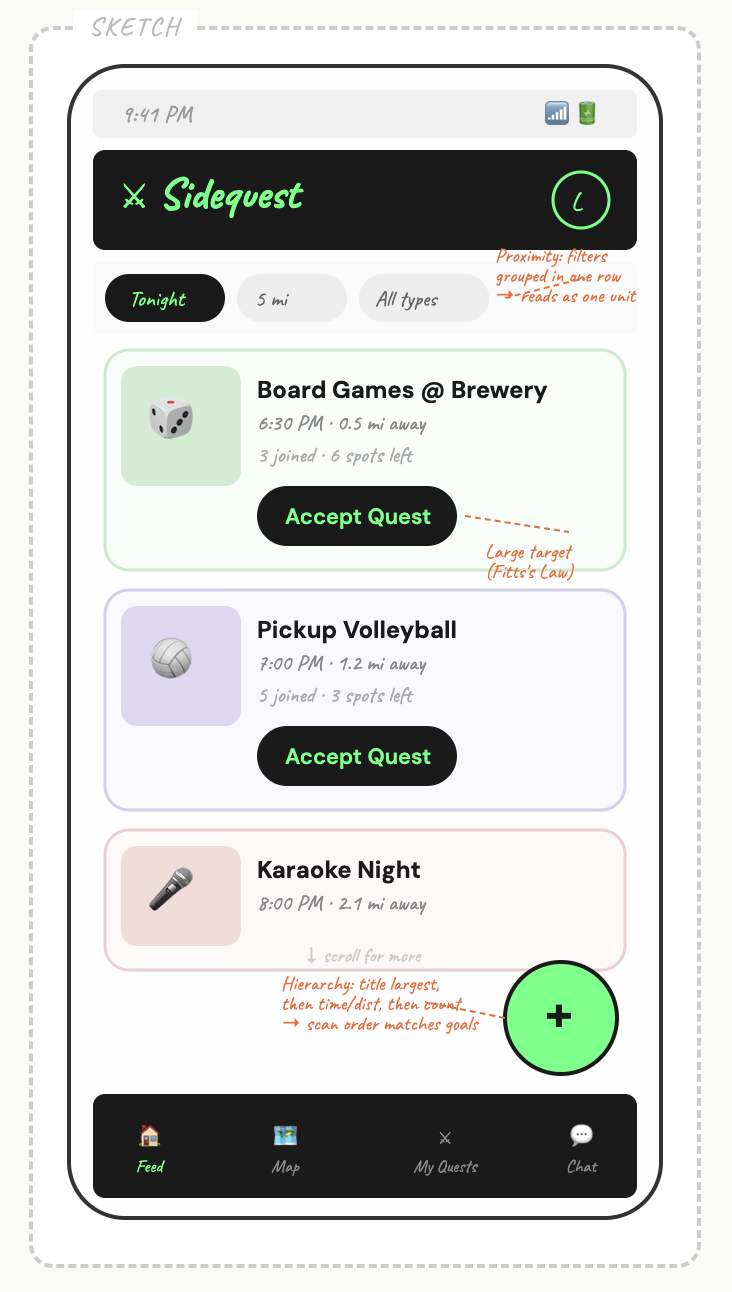
\includegraphics[width=0.7\textwidth]{homescreen_template.png}
\end{center}

\textbf{Layout:} A three-column filter bar (When / Distance / Category) at the top, followed by a vertical scroll of quest cards. Each card shows title, time, distance, location, host, and an ``Accept Quest'' call-to-action button on the right. Summary metrics (Nearby, Open Spots, Joined) sit at the bottom, followed by collapsible charts.

\textbf{Design Annotations:}
\begin{itemize}[nosep]
    \item \textit{Hierarchy:} The quest title is rendered in bold at a larger weight than the metadata caption, so Leo's eye lands on the activity name before the logistical details.
    \item \textit{Fitts's Law (Tognazzini):} The ``Accept Quest'' button is placed at the far right of every card --- reachable with a right-thumb tap on a phone and immediately visible without scrolling within the card.
    \item \textit{Proximity (Gestalt):} The three filter controls are grouped in a single row so they read as one cohesive filter unit rather than three unrelated inputs.
\end{itemize}

\subsubsection{Host a Quest}

\begin{center}
    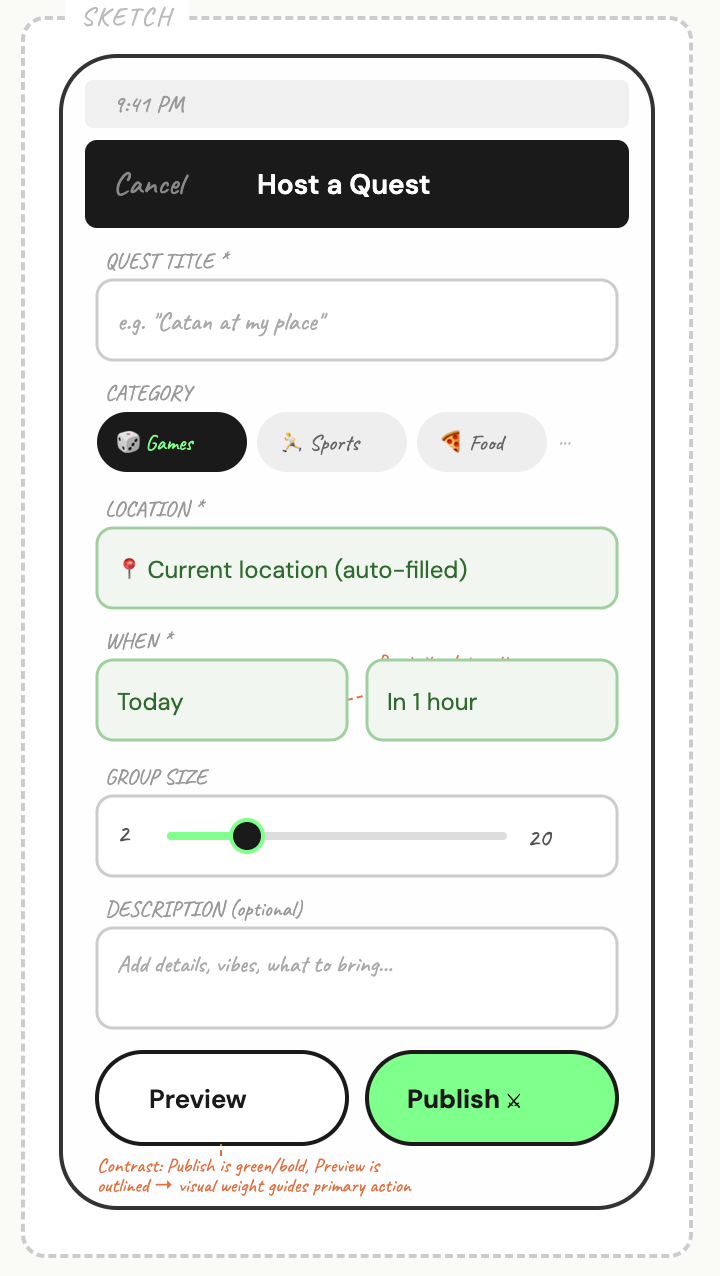
\includegraphics[width=0.7\textwidth]{hostaquest_template.png}
\end{center}

\textbf{Layout:} A top-to-bottom form with labeled fields: Quest Title, Category (horizontal chip radio), Location (auto-filled), When (date + time side by side), Group Cap (slider), and Description. A Preview button and a Publish button sit at the bottom.

\textbf{Design Annotations:}
\begin{itemize}[nosep]
    \item \textit{Rams' ``As little design as possible'':} Only the fields necessary to post an activity are shown. Description is explicitly optional to reduce the perceived effort of hosting.
    \item \textit{Consistency (Norman):} The green primary-button style used for ``Accept Quest'' on the feed is reused here for ``Publish,'' ensuring users recognize the call-to-action pattern across pages.
    \item \textit{Feedback (Shneiderman):} A Preview step shows users exactly what will appear on the feed before they commit, directly addressing Leo's anxiety about accidentally publishing incomplete information.
\end{itemize}

\subsubsection{My Quests}

\begin{center}
    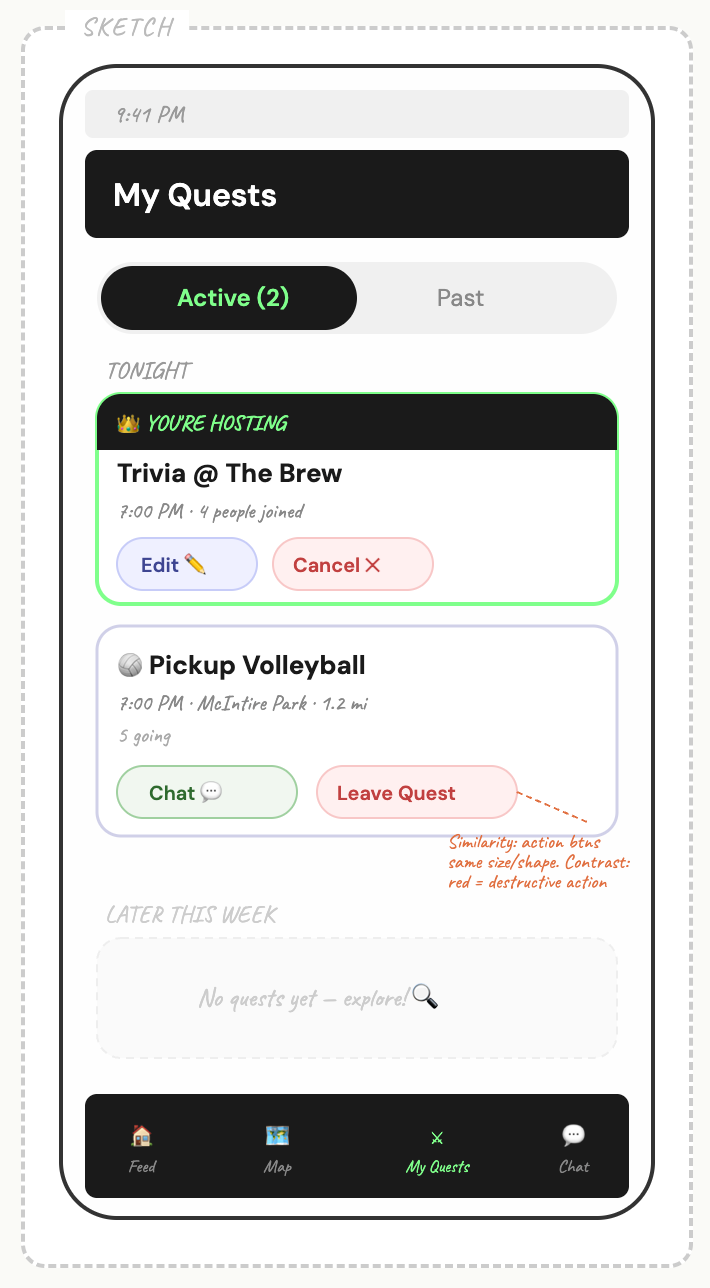
\includegraphics[width=0.7\textwidth]{myquests_template.png}
\end{center}

\textbf{Layout:} A horizontal Active/Past radio toggle at the top. Active view shows two sections: ``Quests You're Hosting'' and ``Quests You've Joined,'' each as bordered cards with a Leave or Manage action. A summary table appears at the bottom.

\textbf{Design Annotations:}
\begin{itemize}[nosep]
    \item \textit{Shneiderman's ``Permit easy reversal'':} Every card has a Leave or Cancel button, making it frictionless to undo a commitment --- the core anxiety point identified in M1.
    \item \textit{Common Region (Gestalt):} Hosting and Joined cards are rendered in visually distinct sections so Leo can immediately understand his role in each activity.
    \item \textit{Whitespace:} Cards are separated with padding and a border, giving each commitment room to breathe rather than collapsing into a dense list.
\end{itemize}

\subsubsection{Group Chat}

\begin{center}
    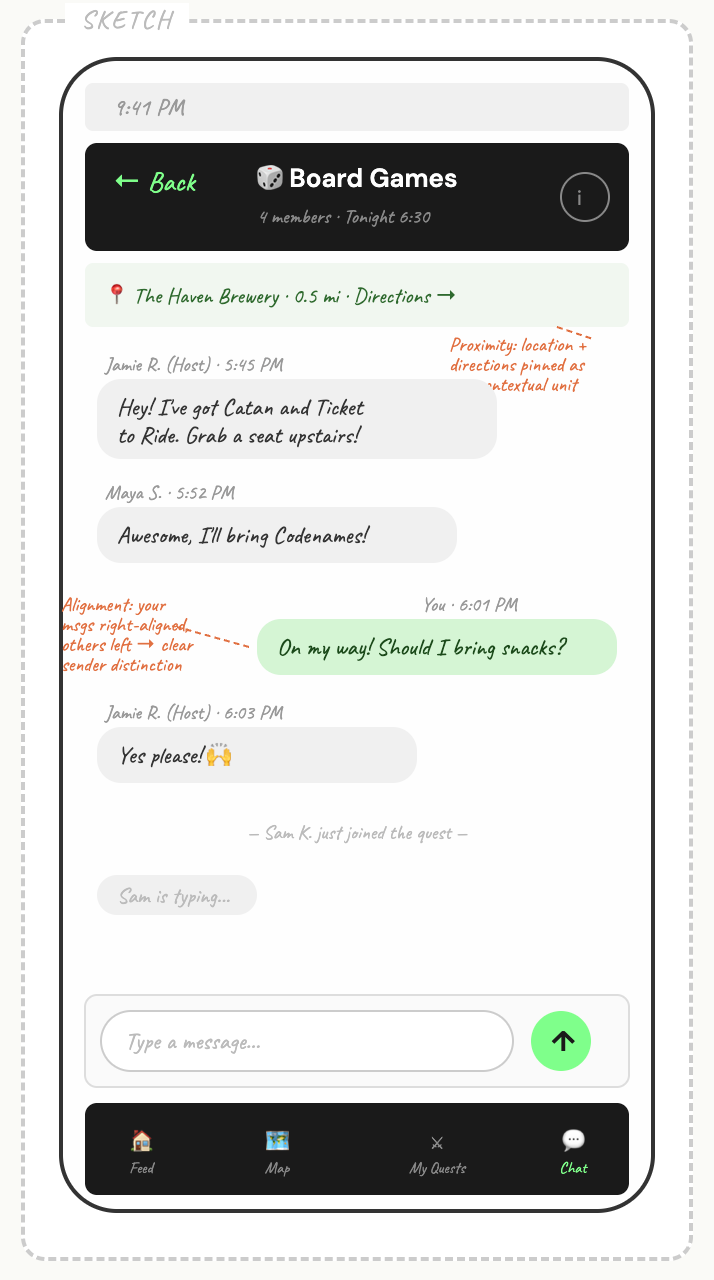
\includegraphics[width=0.7\textwidth]{groupchat_template.png}
\end{center}

\textbf{Layout:} A dark-styled quest header (title, member count, start time) followed by a green location bar with a ``Directions →'' affordance. Chat bubbles alternate between right-aligned (You, green) and left-aligned (others, light gray). A sticky text input with a Send button sits at the bottom.

\textbf{Design Annotations:}
\begin{itemize}[nosep]
    \item \textit{Emphasis via Color Contrast:} Your own messages appear in a green bubble that matches the brand accent; others appear in neutral gray. This immediately distinguishes your messages without labels.
    \item \textit{Figure-Ground (Gestalt):} The dark quest header creates a clear visual separation between context (what quest this is) and content (the actual messages).
    \item \textit{Continuity:} The location bar directly beneath the header keeps the meeting place information visible without the user having to leave the chat to check it.
\end{itemize}

\subsubsection{Quest Detail}

\begin{center}
    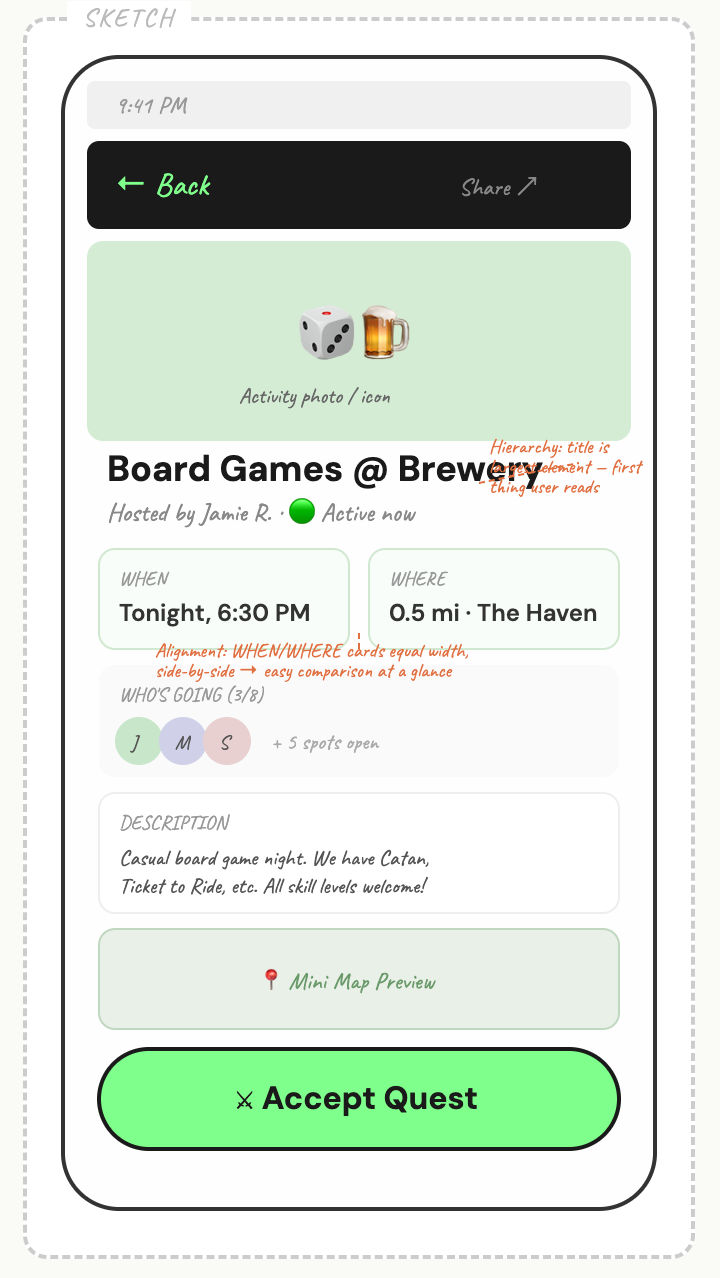
\includegraphics[width=0.7\textwidth]{details_template.png}
\end{center}

\textbf{Layout:} A photo/icon placeholder at the top, followed by the quest title, host, and status. A two-column info row shows When and Where. An expandable Attendees section lists names and roles. Description text follows, then a large full-width Accept Quest or Leave button at the bottom.

\textbf{Design Annotations:}
\begin{itemize}[nosep]
    \item \textit{Fitts's Law:} The call-to-action button spans the full page width and sits at the very bottom of the screen where the thumb naturally rests, minimizing the effort required to commit.
    \item \textit{Hierarchy:} The activity title is the largest text element on the page, followed by host info in regular weight, and metadata in a smaller caption style.
    \item \textit{Closure (Gestalt):} The attendee list is collapsed by default. Users perceive the section as complete even before expanding it, reducing cognitive load on the initial view.
\end{itemize}

% =============================================================================
\section{Working Streamlit Multipage Application}
% =============================================================================

\subsection{Layout and Structure}

The app uses multiple Streamlit layout primitives throughout its five pages:

\begin{itemize}
    \item \textbf{\texttt{st.columns}}: Used on every page. On the Discovery Feed, a three-column row holds the When / Distance / Category filter dropdowns. On Host a Quest, a two-column row places the Date and Time inputs side by side. On My Quests and Quest Detail, \texttt{st.columns([3, 1])} splits card content from action buttons.
    \item \textbf{\texttt{st.expander}}: Used in the Discovery Feed to offer a table view of the filtered quest list, and in Quest Detail to house the attendee roster. This keeps information available without cluttering the main view.
    \item \textbf{\texttt{st.sidebar}}: Streamlit's built-in sidebar navigation provides page switching, replacing the bottom navigation bar sketched in the mobile wireframes.
    \item \textbf{\texttt{st.container(border=True)}}: Quest cards on the Discovery Feed and My Quests use bordered containers to visually separate each activity.
\end{itemize}

All pages include a clear page-level title (\texttt{st.markdown("\# ...")}), section headers (\texttt{st.write("### ...")}), and a consistent max-width of 700px enforced via CSS to keep the layout readable on both desktop and mobile viewports.

\subsection{Input Widgets}

The app includes nine distinct interactive widgets, each meaningfully affecting displayed output:

\begin{enumerate}
    \item \textbf{\texttt{st.selectbox} --- When filter} (Discovery Feed): Filters the displayed quest cards by time window.
    \item \textbf{\texttt{st.selectbox} --- Distance filter} (Discovery Feed): Filters quests by maximum distance in miles.
    \item \textbf{\texttt{st.selectbox} --- Category filter} (Discovery Feed): Narrows the feed to a single activity type or shows all.
    \item \textbf{\texttt{st.text\_input} --- Quest Title} (Host a Quest): Required field that enables the Publish button; drives the quest card content written to session state.
    \item \textbf{\texttt{st.radio} --- Category chips} (Host a Quest): Horizontal chip-style category selector that sets the category emoji and label on the new quest.
    \item \textbf{\texttt{st.date\_input} and \texttt{st.time\_input} --- When} (Host a Quest): Together they compose the start datetime shown on the published quest.
    \item \textbf{\texttt{st.slider} --- Group Cap} (Host a Quest): Determines spots\_total on the new quest, which in turn drives the spots-left count visible to other users.
    \item \textbf{\texttt{st.slider} --- Chart distance} (Discovery Feed charts): Dynamically filters the bar chart to show only quests within the selected radius.
    \item \textbf{\texttt{st.multiselect} --- Scatter category filter} (Discovery Feed charts): Filters the scatter plot to selected categories in real time.
\end{enumerate}

\subsection{Performance and Display}

\textbf{Caching:} \texttt{@st.cache\_data} is applied to \texttt{load\_quests()} in the Discovery Feed and to \texttt{load\_quest\_db()} in My Quests, Group Chat, and Quest Detail. Because \texttt{build\_quests()} is seeded with \texttt{random.seed(42)}, the output is deterministic, making caching safe and effective. Without caching, each widget interaction would regenerate the entire quest list, adding unnecessary computation.

\textbf{Data display:} \texttt{st.dataframe} is used in the Discovery Feed's table expander and on the Host a Quest page to show published quests. \texttt{st.table} is used for the summary table on My Quests and the attendee roster on Quest Detail.

\textbf{Feedback messages:}
\begin{itemize}[nosep]
    \item \texttt{st.success} --- shown when a quest is joined or hosted successfully.
    \item \texttt{st.warning} --- shown when no quests match the current filters, and when the user tries to send an empty chat message.
    \item \texttt{st.info} --- shown when the user leaves a quest.
    \item \texttt{st.error} --- shown when a user tries to publish without filling in required fields, and when a quest is full.
    \item \texttt{st.balloons()} --- celebratory animation triggered on join and publish to reinforce the ``fun'' brand tone.
\end{itemize}

\textbf{Metrics:} \texttt{st.metric} is used at the bottom of the Discovery Feed (Nearby, Open Spots, Joined) and on My Quests (Active, Left / Cancelled) and Host a Quest (Total Hosted) to give Leo a quick status summary without having to read through lists.

% =============================================================================
\section{Data Visualizations}
% =============================================================================

Both visualizations are embedded in the Discovery Feed page and built with Plotly Express. They respond dynamically to user controls, directly answering the question Leo is always asking: \textit{``What should I join right now?''}

\subsection{Bar Chart: Open Spots by Category}

\textbf{Chart type:} Vertical bar chart (\texttt{plotly.express.bar}).

\textbf{Control:} A distance slider (\texttt{st.slider}, range 0.5--10 mi) filters the underlying data before aggregation. The chart updates immediately as the slider moves.

\textbf{What it shows:} For the user-selected radius, the total number of open spots across each activity category. Bars are color-coded by category and labeled with the spot count above each bar.

\textbf{Why this chart type:} Bars are ideal for comparing discrete categories side by side. Leo can glance at the chart and immediately see which activity type has the most availability near him --- a direct answer to ``where are the open spots?'' without reading through individual cards.

\textbf{Connection to persona:} Leo's M1 goal is to find low-stakes activities on short notice. Seeing that, say, ``Sports'' has 14 open spots within 2 miles lets him quickly assess whether his preferred activity type has capacity, which informs whether he should bother scrolling the feed for that category.

\subsection{Scatter Plot: Distance vs. Start Time}

\textbf{Chart type:} Scatter plot (\texttt{plotly.express.scatter}).

\textbf{Control:} A multiselect (\texttt{st.multiselect}) lets Leo filter which categories appear on the chart. Dot size encodes the number of spots left (larger = more open), and color encodes category.

\textbf{What it shows:} Each quest is plotted by its distance from the user (x-axis) and its start time (y-axis). Hovering over a dot reveals the quest title, location, host, and start time.

\textbf{Why this chart type:} Scatter plots are ideal for showing the relationship between two continuous variables. This chart helps Leo make the classic spontaneous-activity trade-off: a quest that is closer but starts later versus one that is farther but starting now. No other chart type surfaces this two-dimensional trade-off as clearly.

\textbf{Connection to persona:} Because Leo uses the app in short 2--3 minute bursts and cares about both proximity and immediacy, this chart gives him a spatial summary of the decision landscape in a single glance, reducing the cognitive load of mentally comparing individual cards.

% =============================================================================
\section{Design Justification}
% =============================================================================

\subsection{How Sketches Evolved from Milestone 1}

Our M1 persona, Leo Vance, established three core requirements that directly shaped the sketch phase:

\begin{enumerate}
    \item \textbf{Speed}: open the app and find something to do in under 60 seconds.
    \item \textbf{Proximity + time filtering}: default to ``right now, near here.''
    \item \textbf{Frictionless coordination}: talk to the group without giving out your phone number.
\end{enumerate}

Our M1 heuristic evaluation of Meetup identified three pain points we designed against: excessive navigation depth to reach a ``happening now'' feed (violated H7 Flexibility), a cluttered home screen profile header (violated H8 Aesthetic), and no accessible help or feedback (violated H10 Help). Every sketch decision was a direct response to one of these findings.

The initial sketches were mobile-first mockups imagining Sidequest as a native-style app with a bottom navigation bar, floating ``+'' action button, and modal overlays for the Host form and Quest Detail view. These were the right concepts to validate quickly --- they forced us to think about thumb reach and single-screen density before worrying about Streamlit's component model.

\subsection{Widget Choices}

\textbf{Discovery Feed filter row:} We chose three \texttt{st.selectbox} dropdowns in a \texttt{st.columns(3)} layout rather than a sidebar because Leo uses the app on the go and the feed and its filters should co-exist on one screen. A sidebar would hide the filters behind an extra tap.

\textbf{Host a Quest form:} The Category field uses a horizontal \texttt{st.radio} rather than a second selectbox to make the six categories visible simultaneously without requiring a dropdown open/close interaction. The Group Cap uses a \texttt{st.slider} rather than a number input because dragging a slider is faster than typing, and the range (2--20) is small enough that precision is not needed. Date and time are placed side by side in \texttt{st.columns(2)} to reinforce that they together answer the single question ``When is this?''

\textbf{My Quests toggle:} An \texttt{st.radio} with \texttt{horizontal=True} provides a tab-like Active/Past switch with no extra visual weight, keeping the page header minimal.

\textbf{Group Chat:} A \texttt{st.selectbox} replaces the sketched ``Back'' button for chat switching. Since Streamlit re-renders the entire page on every interaction, there is no navigation stack to go ``back'' in. A dropdown is the honest representation of the available state.

\subsection{Layout and Navigation}

The sidebar navigation provided by Streamlit's multipage structure maps cleanly to Leo's three primary flows: discover → join, host, and coordinate. The page order (Discovery Feed first, Group Chat later) matches the logical sequence of Leo's evening: he finds something, joins it, then talks to the group.

Within pages, controls are consistently placed above content (filters above cards, chat selector above bubbles), which follows Shneiderman's principle that users need to know what options exist before they see results.

\subsection{Chart Selection}

The bar chart answers ``Where is capacity?'' (which category has open spots near me?). The scatter plot answers ``When and how far?'' (should I go to the nearer thing or wait for the more appealing one?). Together they give Leo the two dimensions he needs to make a spontaneous decision without reading every card.

We chose Plotly over Streamlit's native charts because Plotly's \texttt{hover\_data} allows us to surface the quest title and host name on mouseover, turning the charts from passive summaries into active discovery tools.

\subsection{What Changed from Sketches to Implementation}

\begin{itemize}
    \item \textbf{Bottom navigation bar → sidebar:} Streamlit's page routing is sidebar-based. Rather than fighting the framework, we embraced it. The sidebar actually improves discoverability on desktop because all five pages are always visible.
    \item \textbf{Host a Quest modal → full page:} Streamlit does not support complex multi-field modals. Making it a full page allowed us to use the full canvas for the form, which reduced visual clutter per the sketched layout.
    \item \textbf{Group Chat ``Back'' button → quest selector dropdown:} Described above. The dropdown is more honest about the Streamlit rendering model and still lets users switch between multiple chats, which the sketch's back-button navigation would not have supported without additional state management.
    \item \textbf{Quest card photo → text card:} The sketch showed activity thumbnail images on each card. Streamlit's layout model makes image-in-card grids awkward and slow to render. We replaced thumbnails with emoji category labels, maintaining visual variety with no performance cost.
\end{itemize}

\subsection{Trade-offs}

\textbf{Simplicity vs.\ features:} We did not implement location services, authentication, or real-time push updates. These would be essential in a production app but are out of scope for a Streamlit prototype. The mock data generated by \texttt{quest\_data.py} is seeded deterministically so that the demo experience is consistent across reruns, which is more valuable for evaluation than random data.

\textbf{Aesthetics vs.\ functionality:} We applied a small CSS block on every page to unify the green primary button style and enforce a 700px max-width. This is the minimum cosmetic intervention needed to make the app look intentionally designed rather than Streamlit-default. We deliberately avoided more invasive CSS overrides (e.g., hiding the Streamlit header or hamburger menu) because they create fragile, version-dependent hacks.

% =============================================================================
\section{Visual Design Review}
% =============================================================================

\subsection{Detail View}

\textit{Checking: typography, spacing, colors, icon/element alignment.}

\textbf{Observation 1 --- Typography hierarchy is consistent.}
Across all pages, the page title uses \texttt{\#} (H1), section headers use \texttt{\#\#\#} (H3), card titles use \texttt{**bold**}, and metadata uses \texttt{st.caption} (smaller, lighter). This three-level hierarchy is applied without exception, so the visual weight of text always signals its importance accurately. No fixes were needed.

\textbf{Observation 2 --- Green accent color is reserved for primary actions only.}
The \texttt{\#34C759} green is applied exclusively to primary buttons (``Accept Quest,'' ``Publish,'' ``Send''). It does not appear on secondary actions (Preview, Leave, Cancel) or informational elements. This strict semantic use ensures the color carries meaning rather than decoration. During a review pass, we found that the ``View as table'' expander toggle picked up a faint green tint from Streamlit's default focus ring; we confirmed this is a framework default and not our CSS, and left it since it does not cause confusion.

\subsection{Page-Level View}

\textit{Checking: visual hierarchy, alignment, whitespace, content fit.}

\textbf{Observation 1 --- Discovery Feed visual flow is correct.}
The eye enters at the filter bar (widest, top), moves to the ``Nearby · N quests'' caption, then scans quest cards top to bottom. The ``Accept Quest'' button on the right of each card creates a consistent vertical rhythm along the right edge, making it easy to scan-and-tap down the list. No fixes were needed.

\textbf{Observation 2 --- My Quests page had orphaned ``Summary'' section when the joined list was empty.}
An early version of My Quests rendered the Summary table section even when no quests existed, producing an empty table with headers and no rows. We fixed this by wrapping the summary section in a conditional (\texttt{if st.session\_state.joined\_quests:}), so the section only appears when there is something to show. This eliminates the confusing empty state.

\subsection{Function-Level View}

\textit{Checking: loading states, error states, success states, form validation, navigation awareness.}

\textbf{Observation 1 --- All three feedback states are covered on Host a Quest.}
\begin{itemize}[nosep]
    \item \textit{Error:} \texttt{st.error} fires immediately if the user clicks Publish without a Title or Location.
    \item \textit{Success:} \texttt{st.success} and \texttt{st.balloons()} fire on successful publish.
    \item \textit{Preview:} The Preview button renders an inline card preview so users can verify before committing --- a ``dialog closure'' pattern from Shneiderman.
\end{itemize}

\textbf{Observation 2 --- Group Chat empty state guides the user forward.}
When the user has no joined or hosted quests, the Group Chat page shows an explicit message: ``No chats yet. Join or host a quest first --- a group chat gets created automatically.'' This eliminates the blank-page confusion that would occur without an empty state and tells Leo exactly what to do next.

\textbf{Observation 3 --- Filter mismatch produces a warning, not silence.}
When the Discovery Feed's active filters return zero quests, \texttt{st.warning("No quests match your filters. Try widening your search.")} is displayed. Without this, an empty page could be mistaken for a loading error. The warning keeps the user informed and suggests a recovery action (widen the search), consistent with Norman's feedback principle.

\subsection{App-Level View}

\textit{Checking: cross-page consistency, navigation coherence, information architecture.}

\textbf{Observation 1 --- Visual language is consistent across all five pages.}
Every page applies the same CSS block: max-width 700px, green primary button, rounded 24px button corners, and consistent font-weight conventions. As a result, switching pages feels like moving within a single product rather than between five independent scripts. This was not accidental --- we centralized the CSS snippet and copied it to each page's \texttt{st.markdown()} block.

\textbf{Observation 2 --- Session state is initialized defensively on every page.}
Because Streamlit can enter any page directly from the URL, each page re-checks and initializes \texttt{joined\_quests}, \texttt{hosted\_quests}, and \texttt{chat\_messages} if they do not exist. Without this, navigating directly to Group Chat without first visiting the feed would crash the app with a \texttt{KeyError}. This defensive pattern ensures the app behaves coherently regardless of the navigation path taken, which is essential for an app where users may bookmark a specific page.

\textbf{Observation 3 --- Information architecture matches Leo's mental model.}
The page order --- Discovery Feed → Host a Quest → My Quests → Group Chat → Quest Detail --- follows the natural sequence of using the app: find something, create something, manage your commitments, talk to your group, and inspect details. This ordering is not arbitrary; it matches the task flows defined in M1 (Discovering and Joining, Hosting, Bailing on a Commitment) and makes the sidebar feel like a logical guide rather than an arbitrary menu.

\end{document}
